% # Suggested Steps
% Find some data for experiments. You can use all films with titles, directors, actors and other related information. Some other data such as 'Infected cases by COVID-19', 'Stock data', 'Library data' etc. is also fine. But the size should be reasonably large.
% Store the data into a database table. Then use select in SQL to find the films with word "XXX" in titles, and record the execution time.
% Store the data into a file, and then load it into RAM. The data in RAM can be any format you preferred. Design an algorithm to search "XXX" in titles. Record the execution time of your algorithm.
% Some other comparisons and experiments you would like to do. Such as you can reorganize data into some other format for faster retrieval. You are recommended to study the mechanism of DMBS for storing and retrieval
%
% # Basic Requirements
% 1. Clearly and easy understanding design.
% 2. You need to show that you really do the experiments by some experimental details and reasonable analysis.
%
% # Bonus
% 1. High concurrency and transaction management
% 2. User privileges management
% 3. Database index and file IO
% 4. Large data sets (the data is large enough and cannot be stored into RAM)
% 5. Compare performance of multiple databases with file system over different operation systems
%
% # References
% 1. https://stackoverflow.com/questions/4279358/pythons-underlying-hash-data-structure-for-dictionaries
\title{数据库管理系统 \\ DBMS}

\maketitle\tableofcontents\clearpage

\section{介绍}
\lipsum[1]



\section{实验设计}
\subsection{实验数据和环境}
原先数据集爬取 \bilibili\ 知名或有争议的 UP 主(具体见附录~\ref{A:config})全部视频下的全部评论,用以做水军等检测,因此数据库课程的 Project 可以拿来直接使用。
但是个人觉得数据集不够完整,因此在数据库建模部分增加用户及视频表格,并通过外键将三张表关联起来。
前期下载数据量有些大,用户数量约五百万,如果将全部用户信息爬下来时间较长,因此放弃。
同时期间有被永久封禁的用户,现在已经找不到其个人信息,所以数据库建模时用户信息省略,仅保存其 uid。
当然为了以后研究方便,并未取消用户表格,所以数据库中共有三张表格:\verbbox{User}、\verbbox{Video}、\verbbox{Comment}。
数据库建模可视化如图~\ref{F:workbench-model},同时利用数据库对象关系映射\cite{sqlalchemy2020sqlalchemy}进行数据库建模,但是为进行跨文件系统的查询,因此有不符合范式的地方,数据库采用 \texttt{PostgreSQL}、\texttt{MySQL} 与 \texttt{SQLite},具体代码见附录~\ref{A:database}。

\begin{figure}[H]
    \centering
    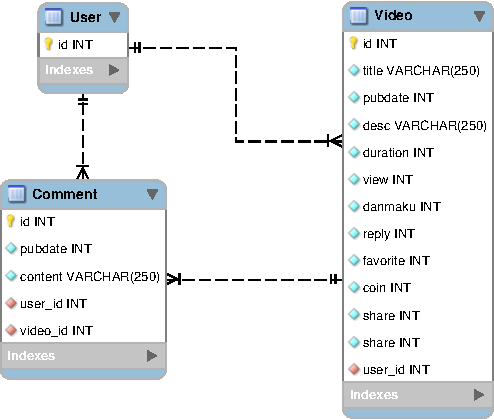
\includegraphics[width=.5\textwidth]{figures/1.pdf}
    \caption{Workbench 数据库模型}\label{F:workbench-model}
\end{figure}

所有数据分为三个文件夹,分别存储用户信息、视频信息以及评论信息,用户信息文件夹仅保存 UP 主的信息及出现在评论区全部用户的 uid,例如:
\begin{python}{users/546195.json}
{"name": "老番茄", "sex": "男", "face": "http://i2.hdslb.com/bfs/face/bc5ca101313d4db223c395d64779e76eb3482d60.jpg", "sign": "新浪微博:_老番茄_", "level": 6, "birthday": "08-13", "archive_view": 909097528, "article_view": 0, "likes": 37261387, "following": 1, "follower": 9548766}
\end{python}
视频信息文件夹保存全部视频的信息,例如:
\begin{python}{videos/av84887919.json}
{"pic": "http://i2.hdslb.com/bfs/archive/202bc40ecf4991d21df91f52a2d112eddb977de1.jpg", "title": "最强自夸王!!!!!", "pubdate": 1579924812, "desc": "歌曲:《自夸小队》\n作词/演唱:某幻君,老番茄,中国boy超级大猩猩,花少北\nHOOK:茶理理理子\n编曲:Lglywww \n混音:Blue coat\n摄影:藤井旋风,大饼\n后期:藤井旋风", "duration": 231, "owner": 1577804, "view": 11436611, "danmaku": 224768, "reply": 26880, "favorite": 530197, "coin": 989930, "share": 130342, "like": 956804}
\end{python}
评论信息文件夹按照视频通过嵌套字典保存保存全部评论信息,第一层的键为用户的 uid,第二册的键为时间戳,第二层的值为评论内容,后期更新代码可以保存评论的全部信息,但是本次 Project 仅考虑用户及时间戳,例如:
\begin{python}{comments/av3051327.json}
{"585481": {"1444662778": "作为天天刷太平洋的刷子团,今天在运送车队这个准备任务上载跟头了,来看看妹子的抢劫放松一下"}, "10917828": {"1444665830": "这期有点恶意卖萌    不过还好  反正我看了"}, "8872386": {"1444671846": "么么哒(`・ω・´)"}, "342211686": {"1581531133": "考古[呲牙][呲牙]"}, "29407696": {"1530278286": "考古"}, "3999038": {"1444689968": "来顶(づ ●─● )づ"}, "7266479": {"1444661483": "44444444先投币点赞在说"}, "495569": {"1444661357": "第三(`・ω・´)"}, "5713034": {"1444659325": "第二^_^"}, "2812699": {"1444658015": "第一(⌒▽⌒)"}, "6306456": {"1497997152": "╮( ̄▽ ̄)╭"}, "15514305": {"1493999905": "考古(=・ω・=)感觉每天就指紫雨视频活了"}, "10954013": {"1547426274": "๑乛◡乛๑"}, "74234761": {"1535518362": "考古"}}
\end{python}

数据库中的用户表格共有 5890919 行数据,视频表格共有 24742 行数据表格,评论共有 34097426 行数据。
全部的程序见 \href{https://github.com/Iydon/homework/tree/master/CS307}{GitHub},至于 \bilibili\ 工具类例如兼容 bv 索引的爬虫见 \href{https://github.com/iydon/bilibili}{GitHub},预计 2020 年 4 月 1 日开源。代码使用 \texttt{Python} 语言,通过 \texttt{pipenv} 进行虚拟环境管理,具体见附录~\ref{A:config}。


\subsection{实验细节}
\lipsum[3]


\subsection{实验结果}
\lipsum[4]



\section{结论}
\lipsum[5]



\section{附加内容}
\lipsum[6]



\clearpage
\section{参考文献}
\nocite{*}
\printbibliography[heading=none]



\clearpage
\begin{appendices}
    \section{配置文件}\label{A:config}
        \pythonfile{../Pipfile}{Pipfile}
        \pythonfile{code/config.py}{config.py}
    \section{数据库建模}\label{A:database}
        \pythonfile{code/database.py}{database.py}
\end{appendices}
